%%%%%%%%%%%%%%%%%%%%%%%%%%%%%%%%%%%%%%%%%%%%%%%%%%%%%%%%%%%%%%%%%%%%%%%%
%%%%%%%%%%%%%%%%%%%%%%%%%%%%%%%%%%%%%%%%%%%%%%%%%%%%%%%%%%%%%%%%%%%%%%%%
\section{Introduction}
This paper focuses on introduction to an amazing world of liquid crystals (\emph{LC}) and simple application of them in \emph{LCD} (liquid crystal display), because nowadays LC panels are still first choice of most companies involved with visualisation and displays.

Basic principle of liquid crystal is, as the name suggests, that it has a structure of a crystal and also can change its shape and structure as a liquid. Major reason of LC dominance is the fact, that the structure change can happen only according to voltage applied, with no mechanics involved. More detailed explanation of it is in chapter \ref{sec:genchar}. 

In LCDs, the ability of liquid crystals to rotate the plane of polarized light is exploited. Using polarizing filters, we can control the intensity of light not blocked by adjusting the voltage. This ability is also used in hyperspectral imaging, for example the infrared camera. There is a lot of other applications of liquid crystals, but in this paper we are focusing on explanation, how TN LCD works, because this is crucial application of LC.

In chapter \ref{sec:history}, long history of liquid crystals research is briefly described. Chapters \ref{sec:genchar} and \ref{txt:charsForLCD} focus on characteristics and properties, mostly those useful for us. That knowledge is later applied in creation of TN LCD cell, which is described in chapter \ref{sec:tnlcd}. Last chapter, \ref{sec:conclusion}., contains conclusion of this report and expected future of LC use.

%%%%%%%%%%%%%%%%%%%%%%%%%%%%%%%%%%%%%%%%%%%%%%%%%%%%%%%%%%%%%%%%%%%%%%%%
%%%%%%%%%%%%%%%%%%%%%%%%%%%%%%%%%%%%%%%%%%%%%%%%%%%%%%%%%%%%%%%%%%%%%%%%
\section{History}
\label{sec:history}
Liquid crystals were studied for long time, before first LCD display came. First observations of this state of matter were made in the second half of the 19th century. Scientists discovered that some materials, for example cholesteryl benzoate, exhibit strange mesophase between solid and liquid state, which can be created by heating this material to a temperature between $145,5\,^{\circ}\mathrm{C}$  and $178,5\,^{\circ}\mathrm{C}$. \cite{kawamoto2002history} One of the scientist were an Austrian botanist, Friedrich Reinitzer, who after the discovery contacted physicist Otto Lehmann and both of them continued this research.

Reinitzer presented his results at a meeting of the Vienna Chemical Society later in 1888. By that time, he had discovered and described three important features of cholesteric liquid crystals: the existence of two melting points, the reflection of circularly polarized light, and the ability to rotate the polarization direction of light. Taken from \cite{wikihistory}. At this point Reinitzer stopped his research and only Lehmann continued and came up with the name \emph{liquid crystals} in 1904.

During the first half of the 20th century, very few people studied liquid crystals and almost nobody showed interest in them. Despite that, some progress was made. French crystallographer Georges Friedel has determined phases of crystals dependent on temperature, as \emph{nematic}, \emph{smectic} and \emph{cholesteric} (see part \ref{txt:lcPhases}). And German chemist Daniel Vorländer had synthesized most of the liquid crystals known.

After the World War II, research in the Europe and United States was renewed and it was obvious that material with liquid crystal properties at room temperature was needed. Among others, one of these substances was synthesized by Hans Kelker at 1969 and his material is most widely researched. In the sixties, flat panel electronic displays were the topic of research and compounds with nematic phase at room temperature made it widely accessible for commercial products.

Around the year of 1970 Swiss company Hoffmann-La Roche filed patent for twisted nematic effect (TN-effect), which was the moment when LCDs became practical. With this invention, first digital quartz wrist watches were soon realizable, by Swiss manufacturers. Japanese companies Sharp and Casio, mainly focused on using first TN panels in calculators and they were "selling like hot cakes" as described in \cite{kawamoto2002history}.

However at this point, each segment of the display was addressed directly, therefore there were limitations of size of panel. As a solution LCD, which used active matrix addressing scheme, was made. This scheme is nowadays used almost by every display in computers, TVs or smartphones.

During the 1970s and 1980s focus were on improving TN-panels, for example a super-twisted nematic display (STN) from 1983. As an alternative to TN LCDs in 1990 the plane switching technology (IPS) was invented. Hitachi improved this new type of display and in 1992 became one of the first manufacturers of IPS LCDs.

At this time, everything was ready for worldwide domination of LC displays. As time passed manufacturers like Samsung, were improving these technologies and made larger displays with bigger pixel density, which trend is continuing to the present.

%%%%%%%%%%%%%%%%%%%%%%%%%%%%%%%%%%%%%%%%%%%%%%%%%%%%%%%%%%%%%%%%%%%%%%%%
%%%%%%%%%%%%%%%%%%%%%%%%%%%%%%%%%%%%%%%%%%%%%%%%%%%%%%%%%%%%%%%%%%%%%%%%
\section{General characteristics}
\label{sec:genchar}
In this section the general characteristics of liquid crystals will be described. More detailed insight into specifics essential for manufacturing and utilization of LCDs can be found in section \ref{txt:charsForLCD}.

%======================================================================%
\subsection{State of matter}
The name \textit{liquid crystal} itself raises the question how a crystal, a compound known to be strictly solid, might posses the features of a liquid. The matter is generally classified into phases by the ability of single molecules to move with respect to each other. Among well defined phases the solid, liquid and gaseous phase can be found. However, under certain conditions, the matter might get into a transitional state where it shows the features of both phases in question. 

A liquid crystal is thus a state of matter representing transition between solid and liquid phase. Even though a liquid crystal phase can be further divided into more specific phases in general the two most important features it adopts from both adjacent basic phases are structural ordering of molecules and the ability to flow like a liquid \cite{Fujitsu2006Online}.

%======================================================================%
\subsection{LC phases} \label{txt:lcPhases}
The matter which is able to achieve the features of liquid crystal consists of anisometric rod-like molecules with one axis significantly longer then the other two \cite{Gu2011WorldofLCD}. Their position and orientation plays key role in the way the light propagates through such a matter and this feature is utilized in LCD displays (as described in section \ref{txt:charsForLCD}).

Liquid crystal can exist in one of many different phases that differ in the positional order and orientation of the molecules. To remain in the specific phase the liquid crystal must meet certain conditions. From this point of view the liquid crystals can be classified as \textbf{thermotropic} or \textbf{lytropic} \cite{Desimpel2006LCD} (and even more categories can be found). The phase of thermotropic LCs depends of the temperature while the the phase of lyotropic LCs depends on their concentration in an isotropic solvent.

The LCs used to manufacture LCDs belong to thermotropic category. Depending on the temperature these crystals can exist in \textbf{isotropic}, \textbf{nematic}, \textbf{smectic} or even more complicated phases \cite{Desimpel2006LCD} (see Figure \ref{fig:lc_phases}). In the isotropic phase single molecules are positioned and oriented arbitrarily, in the nematic phase molecules exhibit almost same orientation and in the smectic phase even layered positional order can be seen.

\begin{figure}[hbt]
\centering
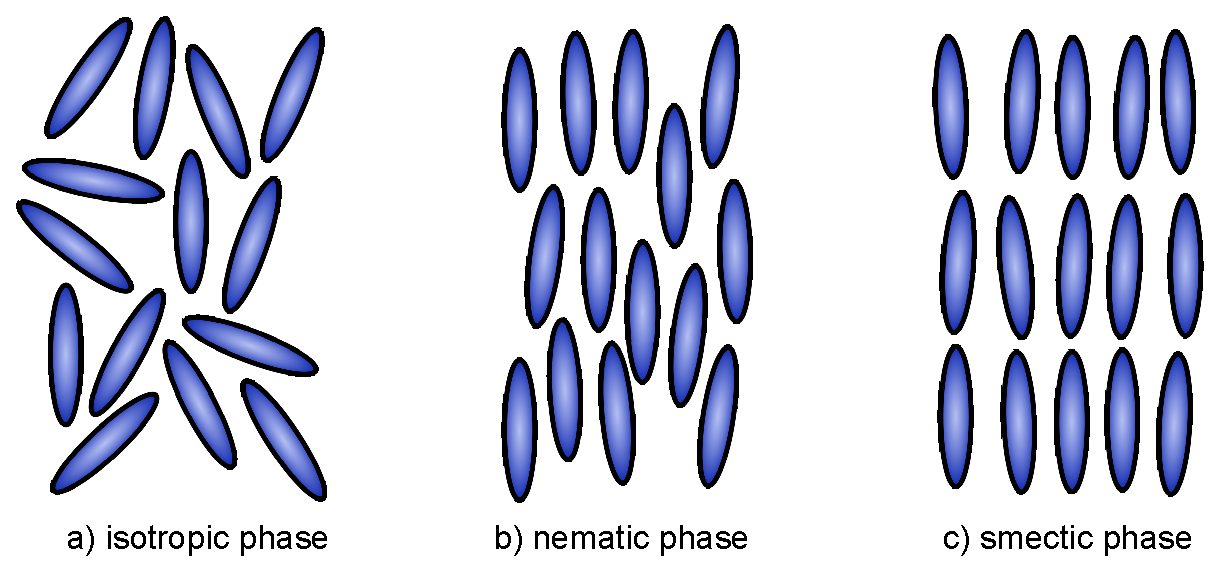
\includegraphics[width=12cm]{img/lc_phases.eps}
\caption{Themotropic liquid crystals phases.}
\label{fig:lc_phases}
\end{figure}


%======================================================================%
\subsection{Orientation of molecules}
In order to easily describe the orientation of the molecules a vector called \textit{director} is defined \cite{Desimpel2006LCD}. This vector represents an average direction of the longest axis of each molecule in specific area of the matter. As for the isotropic phase, the director would strongly differ throughout the medium, while in case of the nematic and smectic phase the director would be aligned very closely with the longest axis of each molecule throughout the whole medium.

%%%%%%%%%%%%%%%%%%%%%%%%%%%%%%%%%%%%%%%%%%%%%%%%%%%%%%%%%%%%%%%%%%%%%%%%
%%%%%%%%%%%%%%%%%%%%%%%%%%%%%%%%%%%%%%%%%%%%%%%%%%%%%%%%%%%%%%%%%%%%%%%%
\section{Characteristics essential for LCD design} \label{txt:charsForLCD}
Liquid crystals exhibit specific features that the whole LCD manufacturing concept builds on \cite{CWRU2011PolymersAndLC}. Primarily the effect of birefringence must be mentioned since it serves the purpose of a polarization filter. What is more the molecules of liquid crystals are susceptible to change their orientation according to the external electrical field. The orientation can be even altered using the material with specially modified surface structure that is in the contact with the outer layer of liquid crystal substance. All of these principles will be described in more detail in the following sections. It should be mentioned that only nematic liquid crystals will be considered.

%======================================================================%
\subsection{Polarization}
The influence of relative direction between director and electric field on the dielectric constant causes another phenomena called \textit{birefringence}. The (unpolarized) light propagating through the liquid crystal experiences two different refractive indexes and thus splits into two separate linearly polarized waves \cite{Gu2011WorldofLCD}. The LCD design does not actually use the birefringence itself but it is based on the fact that liquid crystals posses the ability to control the polarization of the incident light wave. Section \ref{sec:tnlcd} discusses how to rotate the linearly polarized light using twisted nematic liquid crystal cell.

%======================================================================%
\subsection{Electric field}
Due to the anisometric rod-like shape the molecules of liquid crystals cause that the externally applied electric field experiences different dielectric constant when the direction of the electric field vector is parallel or perpendicular to the liquid crystal director. As a result the director tends to align with the electrical field to the extent given by the magnitude of electrical field \cite{Desimpel2006LCD} (see Figure \ref{fig:director}). This phenomena is of the great importance to the basic principle of LCD design.

\begin{figure}[hbt]
\centering
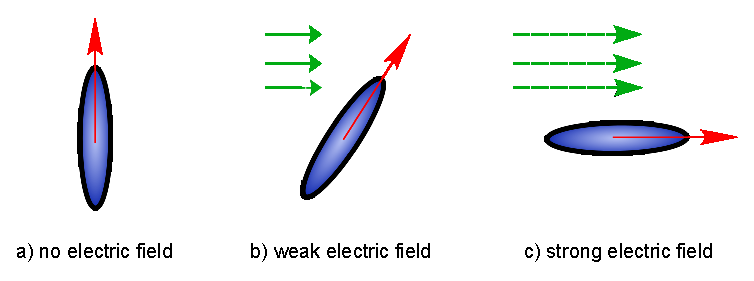
\includegraphics[width=12cm]{img/director.eps}
\caption{Director orientation (red solid arrow) when the external electric field (green dashed arrow) is applied.}
\label{fig:director}
\end{figure}

%======================================================================%
\subsection{Surface structure} \label{txt:surface_structure}
As far as LCD design is concerned it is necessary to obtain a liquid crystal substance with a given (preset) director distribution \cite{Desimpel2006LCD}. Therefore the liquid crystals are usually kept in a thin layer placed between two glass planes. But how to control the default orientation of the director?

This can be achieved by enclosing the liquid crystal layer between two glass substrates with specifically adjusted surfaces. A thin polymer\footnote{For instance nylon or polyvinyl alcohol.} layer is placed on the glass substrate and it is then rubbed in the required direction. The molecules of liquid crystals in contact with such a surface tend to align their directors parallel to the direction of rubbing \cite{DesimpelLCandPhoytonics}.

Let's imagine that the layer of liquid crystals actually consists of sub-layers with the thickness of one molecule. The molecules in each layer align their directors in the same direction while influencing the direction of the directors in the layer beneath and above. 

If both of the glass substrates enclosing the liquid crystal layer are rubbed in the same direction the average direction of the director in each layer will be the same. If the directions of rubbing on both glass substrates are perpendicular to each other the sub-layers of liquid crystals would "rotate" effectively creating the helix structure as can be seen in Figure \ref{fig:director_prerotation}. 

\begin{figure}[hbt]
\centering
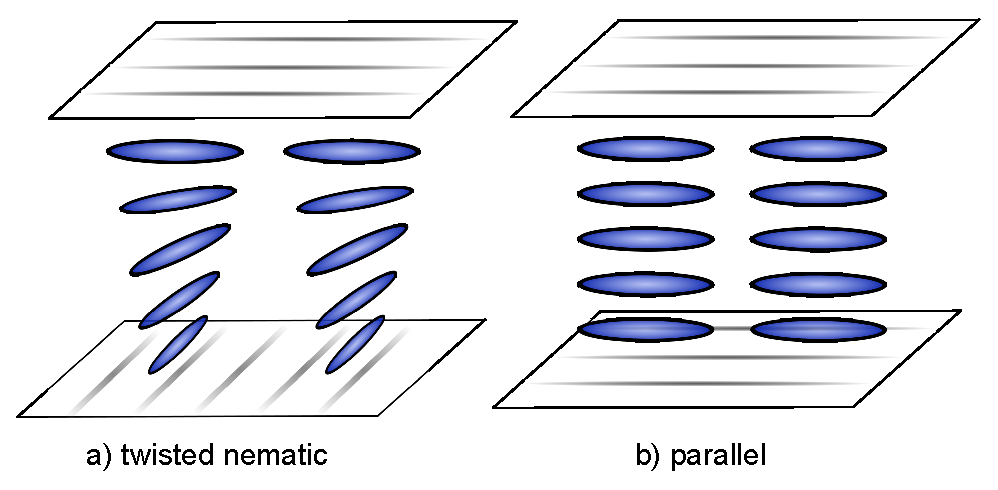
\includegraphics[width=12cm]{img/director_prerotation.eps}
\caption{Liquid crystals layer placed between two glass substrates that have their inner surfaces coated with polymers. Twisted nematic variation can be seen on the left where the directions of rubbing of each glass's plane surface are perpendicular to each other. The right part of the picture shows the parallel variation.}
\label{fig:director_prerotation}
\end{figure}

The latter formation is called \textit{twisted nematic} and represents the essential principal in design of TN LCD.

%%%%%%%%%%%%%%%%%%%%%%%%%%%%%%%%%%%%%%%%%%%%%%%%%%%%%%%%%%%%%%%%%%%%%%%%
%%%%%%%%%%%%%%%%%%%%%%%%%%%%%%%%%%%%%%%%%%%%%%%%%%%%%%%%%%%%%%%%%%%%%%%%
\section{Simple TN LCD}
\label{sec:tnlcd}
In this section the basic principle of LCD display will be described. Many different approaches exist to manufacture a single LCD cell, however the Twisted nematic (TN) cell is the most widely commercially used one \cite[pg.~57]{lueder2010liquid}. Further text therefore explains the principle of the TN LCD display.

The characteristics described in the previous chapter represent the basic principal of LCDs as the susceptibility of the molecules to reorient themselves according to the electric fields and the ability to control the polarization of light effectively provides the manufacturers with the "tool" to switch the passing light on and off.

Each TN LCD cell actually represents one subpixel\footnote{Colored display where each pixel consists of three (RGB) subpixels is considered.} in an LCD display. Figure \ref{fig:tnLcdcell} shows the whole pixel and it can be seen that each TN LCD cell consists of six main components:

\begin{itemize}
\item color filter (red, green, blue),
\item horizontal linear polarizer,
\item rear glass substrate with horizontal surface rubbing,
\item liquid crystals,
\item front glass substrate with vertical surface rubbing,
\item vertical linear polarizer. 
\end{itemize}

\begin{figure}[hbt]
\centering
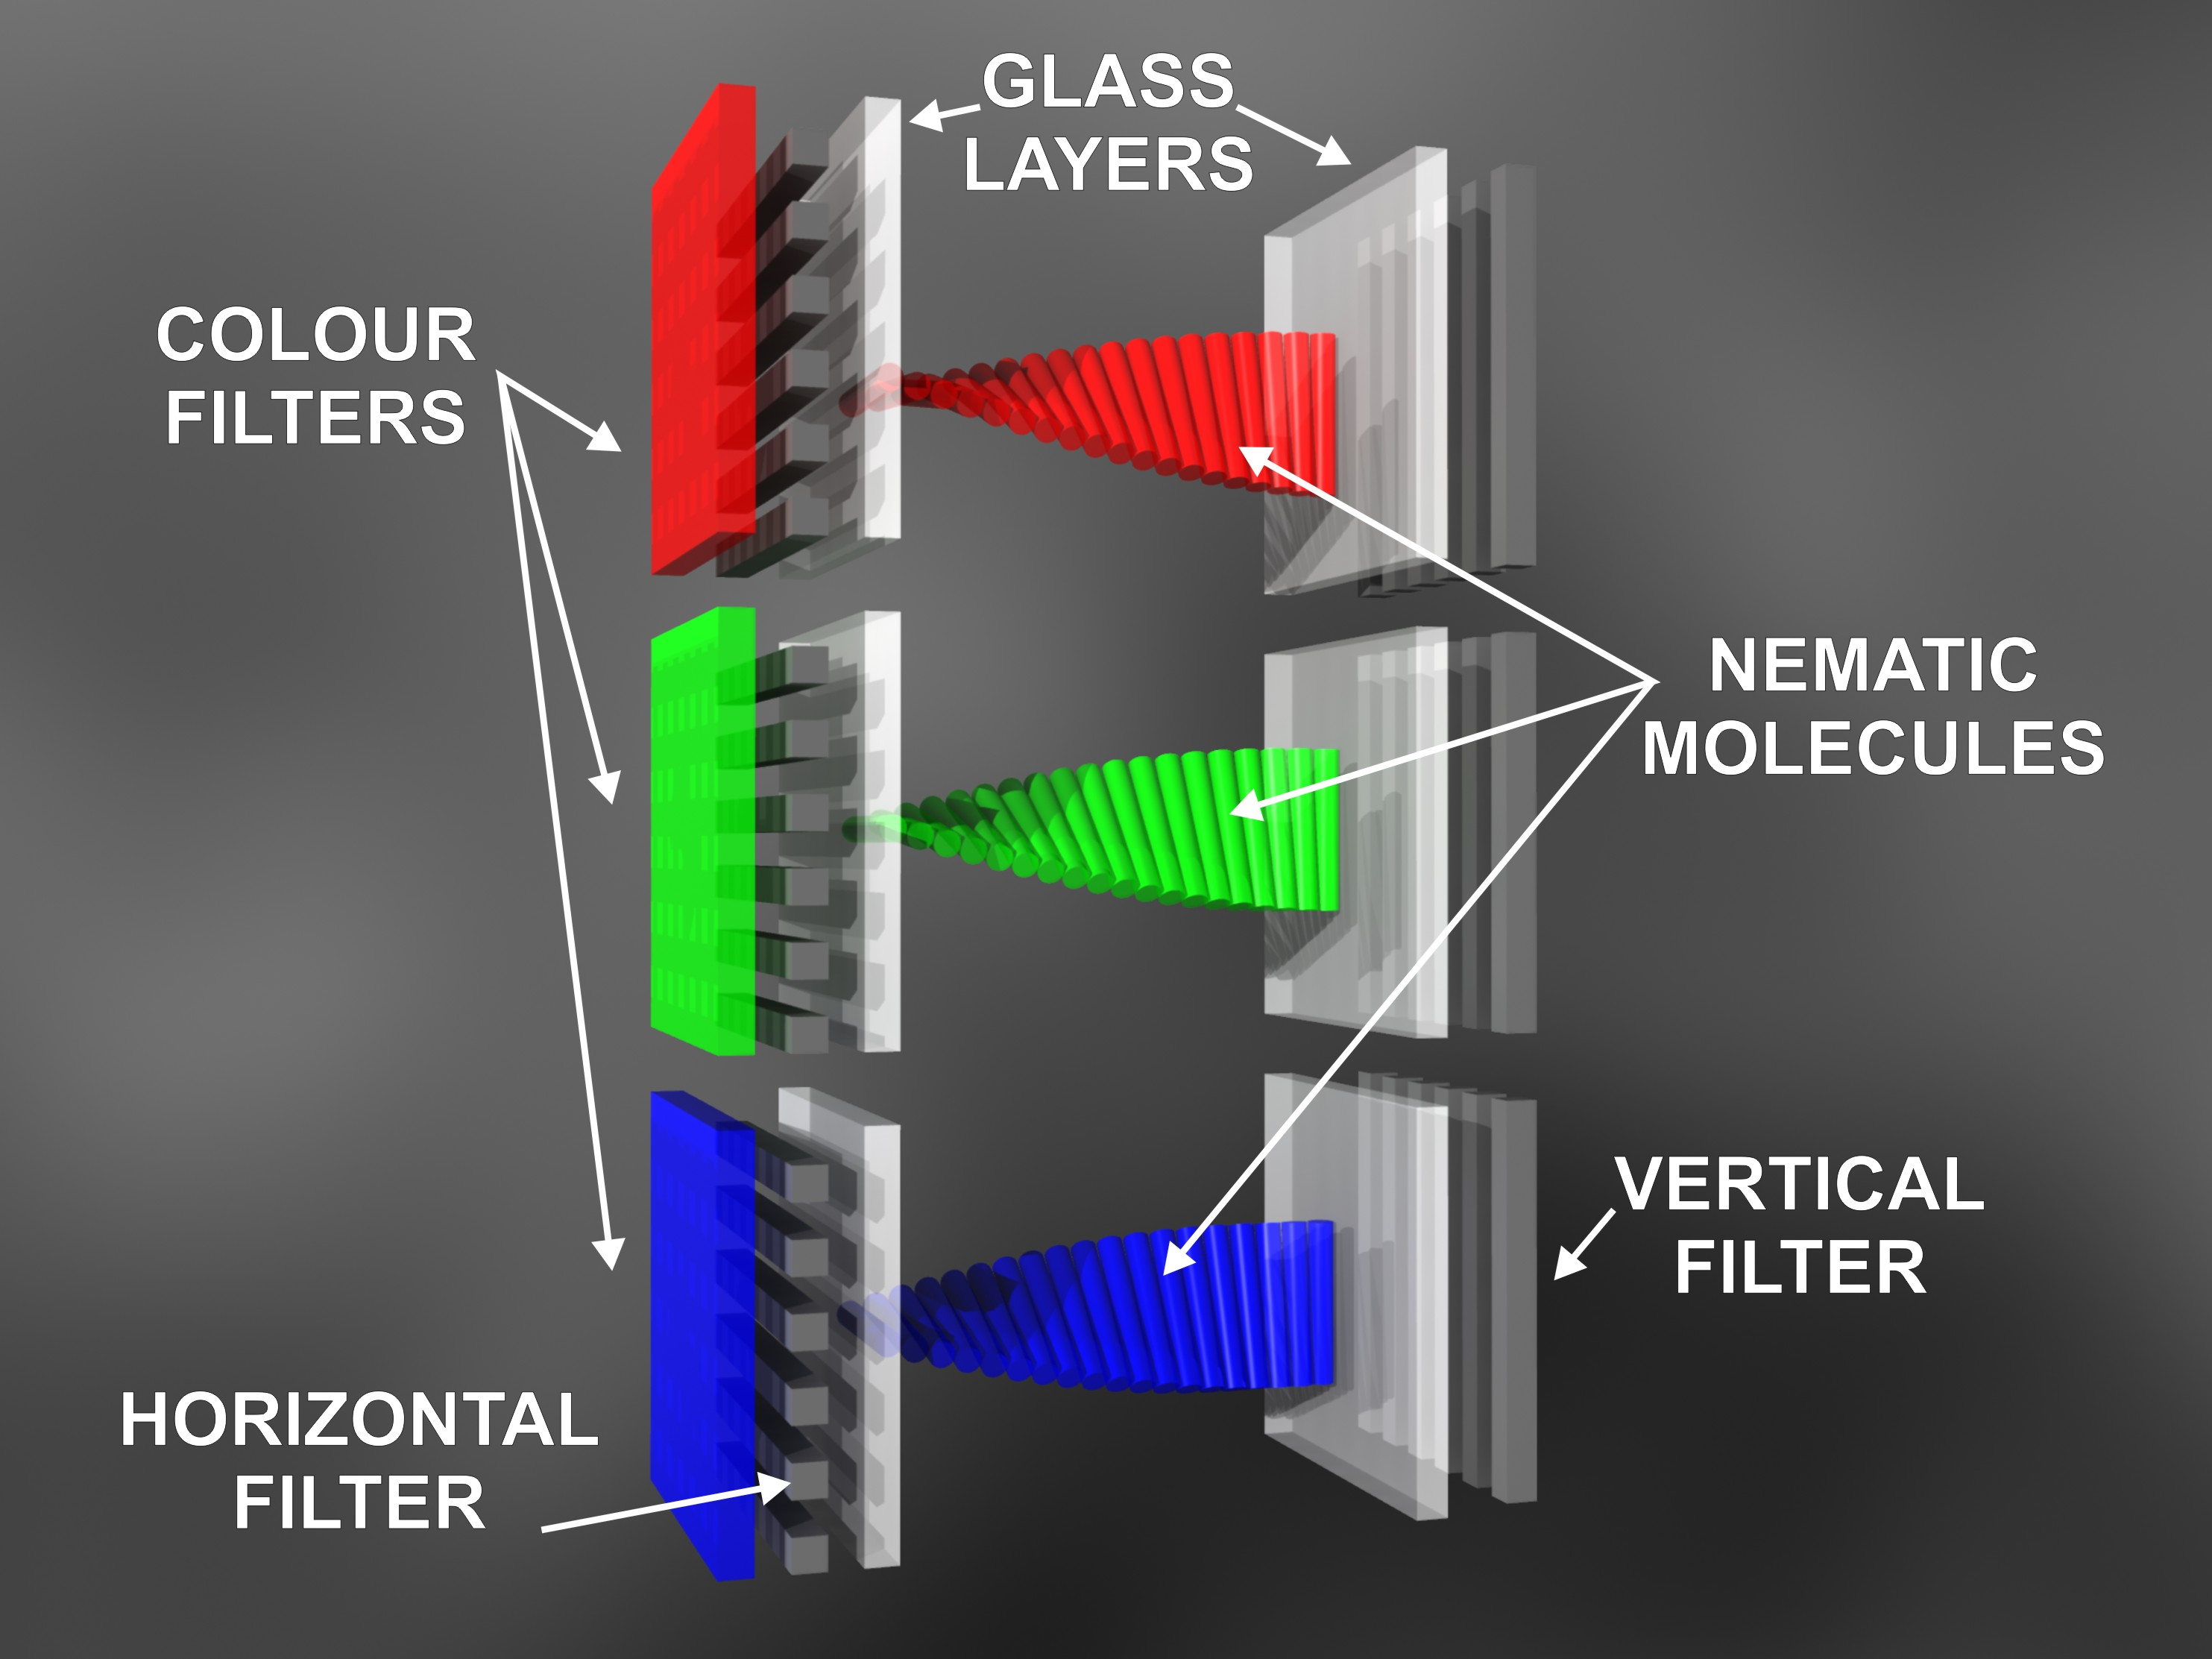
\includegraphics[width=12cm]{img/tn_cell_wiki_en.jpg}
\caption{Three TN LCD cells creating one colored pixel. \cite{tnlcdsubpix}}
\label{fig:tnLcdcell}
\end{figure}

Let's start with the liquid crystals component. As explained in section \ref{txt:surface_structure} thanks to the rubbing applied on both glass substrates the layer of liquid crystals creates the helix structure. Each sub-layer of this structure behaves as the linear polarizer and thus the polarization plane of the light propagating through the cell is rotated along the helix (in this case by 90 degrees).

If the liquid crystals component was missing the (unpolarized) light propagating through the cell would be first linearly polarized thanks to the horizontal polarizer and then absorbed by the vertical polarizer (see Figure \ref{fig:polarizersCrossed}). As the result the observer would see the black rectangle.

\begin{figure}[hbt]
\centering
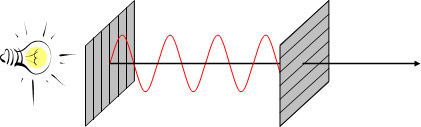
\includegraphics[width=12cm]{img/pol_crossed.jpg}
\caption{Light propagating through two linear polarizers with transmission axes perpendicular to each other. \cite{Desimpel2006polarizersCrossed}}
\label{fig:polarizersCrossed}
\end{figure}

Now let's add the liquid crystal layer between the polarizers. The helix structure of nematic liquid crystals rotates the polarization plain of the light so the beam can easily pass through the second polarizer
(see Figure \ref{fig:polarizersLc}).

\begin{figure}[hbt]
\centering
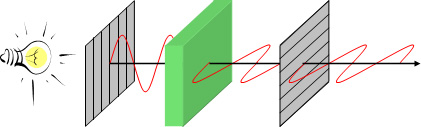
\includegraphics[width=12cm]{img/pol_lc.jpg}
\caption{The layer of twisted nematic liquid crystals is placed between the crossed polarizers. \cite{Desimpel2006polarizersCrossed}}
\label{fig:polarizersLc}
\end{figure}

It si obvious that whether the light passes through the cell or not depends only on the presence of the helix structure. It was already explained that liquid crystals in their nematic phase tend to align their directors parallel to the applied electric field and this is the mean used to control the amount of propagating light. With the increasing voltage applied the helix structure gradually collapses, the incident light experiences the isotropic medium and eventually is absorbed by the second polarizer \cite{Desimpel2006LCD}.

As far as ordinary backlit LCD screens are concerned the magnitude of the voltage applied in order to obtain the full off state varies across different products and manufacturers, the concept stays the same though - no voltage produces the on state (full brightness) while the maximum voltage results in off state (black color).

%%%%%%%%%%%%%%%%%%%%%%%%%%%%%%%%%%%%%%%%%%%%%%%%%%%%%%%%%%%%%%%%%%%%%%%%
%%%%%%%%%%%%%%%%%%%%%%%%%%%%%%%%%%%%%%%%%%%%%%%%%%%%%%%%%%%%%%%%%%%%%%%%
\section{Conclusion}
\label{sec:conclusion}

In this report, basic principles of liquid crystals were explained, along with brief introduction to long and tricky history of liquid crystals research. Authors focused mainly on application in LC displays as it is most commonly seen worldwide these days. Latter chapters describe how crystal reacts in electric field, with differences between all kinds of liquid crystals. Based on these abilities, simple TN panel with one segment is designed and discussed.

Currently there is a big number of different types of LCDs and TN is one of the oldest and simplest variants. Its qualities, like viewing angles and gamut\footnote{Gamut describes how many colors can be accurately represented by a certain output device.}, were surpassed by newer technologies, which are much more complex. In spite of the lack of good properties, TN panels are still used, because they are cheaper and simpler. They are still the best option for displays used for simple office work and specialized devices, like wristwatches and calculators. TN displays are also widely used by players of computer games, for its shortest response time. Overall, this technology is not going to fade away, unless some breakthrough in display development is made.